\documentclass[11pt, pdftex]{article}
\usepackage[margin=1in]{geometry}
\usepackage{graphicx}
\usepackage{amsmath}
\usepackage{listings}
\usepackage{semantic}
\usepackage[hyphens]{url}
\usepackage[breaklinks]{hyperref}
\usepackage[demo]{graphicx}
\usepackage{subcaption}
\usepackage{hyperref}
\title{Assignment (MiniProject) #3}
\author{Machiry Aravind Kumar}
\date{UCSB}
\begin{document}
\maketitle
\section{Dataset}
\subsection{Seeds Data Set}
This dataset is from UCI Archive: \url{https://archive.ics.uci.edu/ml/datasets/seeds}. Dataset contains various Geometric parameters of wheat kernels measured using a soft X-ray technique. It is non-destructive and considerably cheaper than other more sophisticated imaging techniques like scanning microscopy or laser technology. The problem is to classify these into one of the 3 different classes viz  Kama, Rosa and Canadian. For this Assignment, I selected samples for only 2 classes: Kama (Class label: 1) and Rosa (Class label: 2). Available Features in the dataset are:
\begin{itemize}
\item area A.
\item perimeter P.
\item compactness C.
\item length of kernel.
\item width of kernel,
\item asymmetry coefficient
\item length of kernel groove.
\end{itemize}
\section{Running SVM}
I used SVM package from $\texttt{sklearn}$ module. I used following kernel functions: $\texttt{linear,rbf}$ and   $\texttt{sigmoid}$ with different values of Penalty Parameter(C) which trades off misclassification of training examples against simplicity of the decision surface, in other words this parameter controls over fitting, larger value of C results in over fitting and Kernel coefficient (gamma) which defines how much influence a single training example has. Its clear that, we need to select a kernel function which gives highest accuracy with least C and gamma. The error rates of using different kernel functions with different C and gamma are as shown in Table \ref{tab:kerf}. I selected kernel function $\texttt{linear}$ with $C = 1.4$ and $gamma = 0$ as it gives the best result satisfying our constraints.
\begin{table}
\centering
\begin{tabular}{ | c | c | c | c |}
    \hline
    {\bf Kernel Function} & {\bf C} & {\bf gamma} & {\bf Mean Accuracy}\\ 
    \hline
    rbf & 0.1 & 0 & 50.0\\
	\hline
	sigmoid & 0.1 & 0 & 93.57\\
	\hline
	linear & 0.1 & 0 & 94.28\\
	\hline
	linear & 1 & 0 & 94.28 \\
	\hline
	linear & 1.1 & 0 & 94.42\\
	\hline
	linear & 1.2 & 0 & 95.0\\
	\hline
	linear & 1.3 & 0 & 95.71\\
	\hline
	{\bf linear} & {\bf 1.4} & {\bf 0} & {\bf 96.42}\\
	\hline
	linear & 1.5 & 0 & 96.42\\
	\hline
	linear & 10 & 0 & 96.42\\
	\hline
	\end{tabular}
	\caption{Effectiveness of various Kernel Functions}
    \label{tab:kerf}
\end{table}

\begin{figure}
    \centering
    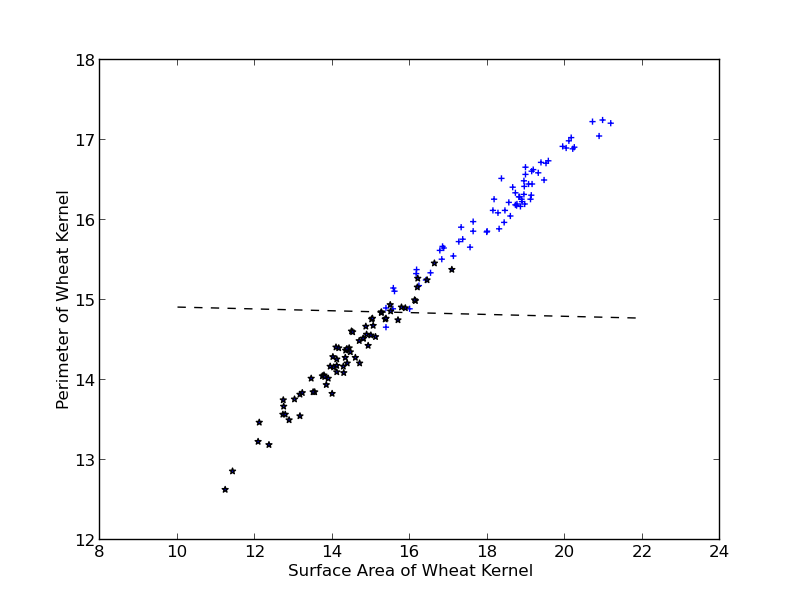
\includegraphics[width=0.6\textwidth]{pics/decbou.png} 
    \caption{Dataset Features with Decision Line}
    \label{fig:decbou}
\end{figure}

\section{Running LDA classifier on the Dataset}
I ran LDA function from sklearn.ida module with default arguments as shown below:

\begin{lstlisting}
classifier = LDA()
classifier.fit(features, classes)

weights = classifier.coef_[0]
dec_s = weights[0] / weights[1]
x = np.linspace(10, 22)

Line Equation:
y = dec_s * x - (classifier.intercept_[0] / weights[1])
\end{lstlisting}

It provided weights and intercept using which I was able to get line equation of the decision boundary. The resulting line equation for Decision boundary is: $\textbf{y = -0.011*x - 15.02}$. Figure \ref{fig:decbou} shows the features with decision line.


\section{Classification Accuracy}
The results for different values of n are as shown in Table \ref{tab:seeds}. The results are pretty accurate with 91$\%$ Accuracy and doesn't vary much with n, which proves that features are good for the classification. It also proves that a linear classifier is good fit for this classification problem.
\begin{table}
\centering
\begin{tabular}{ | c | c | c |}
    \hline
    {\bf N} & {\bf Mean Accuracy} & {\bf Mean Error}\\ 
    \hline
    3 & 91.3 & 8.63\\
	\hline
	4 & 91.99 & 8.00\\
	\hline
	5 & 91.42 & 8.57\\
	\hline
	6 & 91.16 & 8.83\\
	\hline
	7 & 91.42 & 8.57\\
	\hline
	8 & 90.97 & 9.02\\
	\hline
	9 & 90.97 & 9.02\\
	\hline
	10 & 91.42 & 8.57\\
	\hline
	\end{tabular}
	\caption{Cross Validation Results for Seeds Dataset using LDA}
    \label{tab:seeds}
\end{table}
\end{document}